
``Remote Sensing'', simply defined as the observation of geographic features and phenomena from a distance, was first coined by Ms. Evelyn Pruitt in the early 1950s. Pruitt, a geographer in the U.S. Navy's Office of Navel Research, felt there was a need to assign a name to the field of study extensively used in World War II, due the rapid advancement of the imaging capabilities of cameras and scanners at the time. Today, remote sensing is defined as the practice of deriving information about Earth's land and water surfaces using images acquired from an overhead perspective, generally satellites or aerial shots. This is done through the detection of electromagnetic radiation reflected and emitted from the Earth's surface and atmosphere \cite{campbell2011introduction}. 

%A few key events will be described in this report to trace back the roots of remote sensing. \cite{campbell2011introduction}

\subsection{A Brief History of Satellite Remote Sensing and Landsat}
In the early 1800s, photosensitive chemicals were proposed for use in experiments to capture images. Several decades later in 1839 the preliminary results of these investigations were publicly reported by one of the founding fathers of photography, Louis Daguerre. This date forms the convenient arbitrary milestone for the birth of photography. The first aerial photograph milestone has generally been accredited to Gaspard F\'elix Tournachon, in 1858 when he acquired an aerial photograph from a camera tethered to a balloon in France. Over the years, numerous improvements were made to photographic technology, balloons and kites \cite{campbell2011introduction}. 
\par
In World War I, cameras were placed on aeroplanes for reconnaissance. Then, during the the height of Cold War, the U.S. Government developed imaging satellites using specialised photographic film. An example of this is the CORONA photo-satellite resonance system launched in 1960 due to the suspension of U-2 spy plane. Figure 1 shows main recognisance system of the CORONA after deployment \cite{CORONA}. 
\par



%Modern day remote sensing and satellite imaging goes beyond military or strategic applications. As of September 1$^{st}$ 2021, there are 4,550 known operational satellites of which 1030 are for Earth observation \cite{Sat_Data}. Satellite imaging has a major applications in a wide range of industries from monitoring crop growth to forecasting weather.
%This report will focus on cloud cover over Earth, weather forecasting and terrain identification. 


\begin{figure}[H]
\centering
%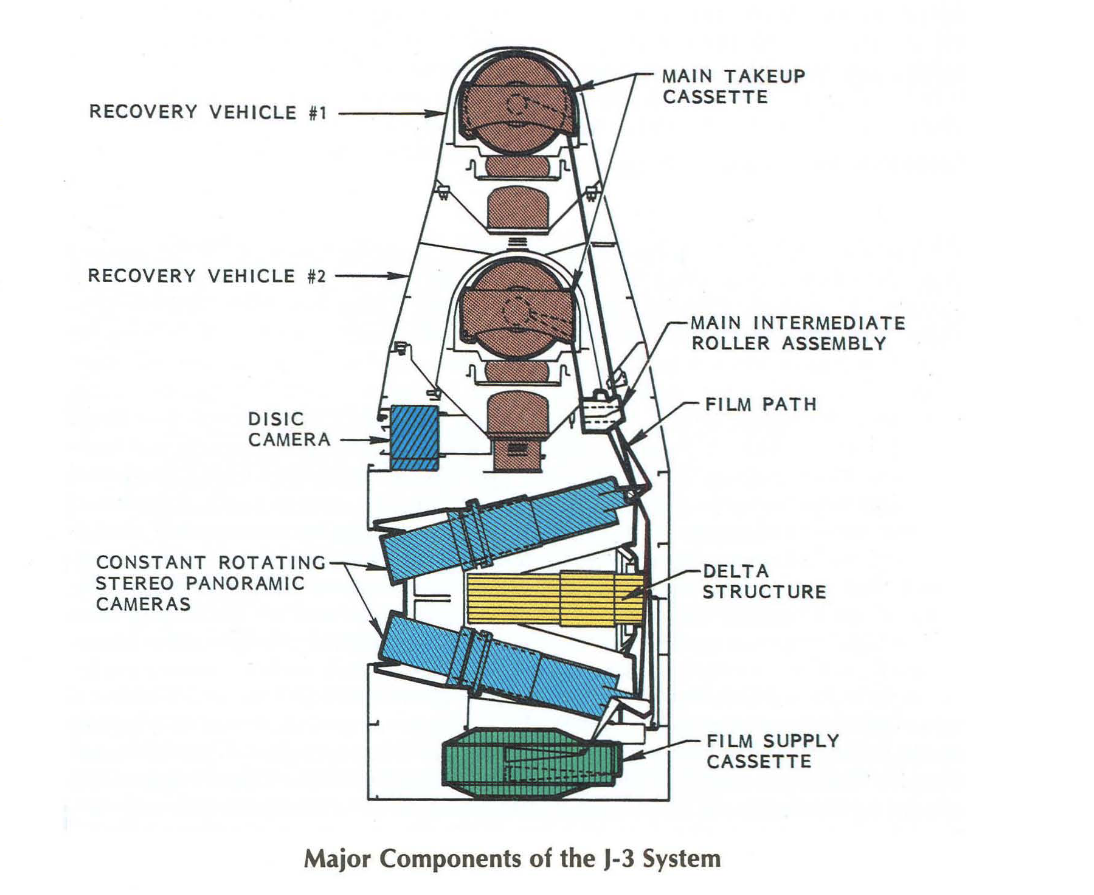
\includegraphics[totalheight=0.3\textheight]{j-3_system.png}
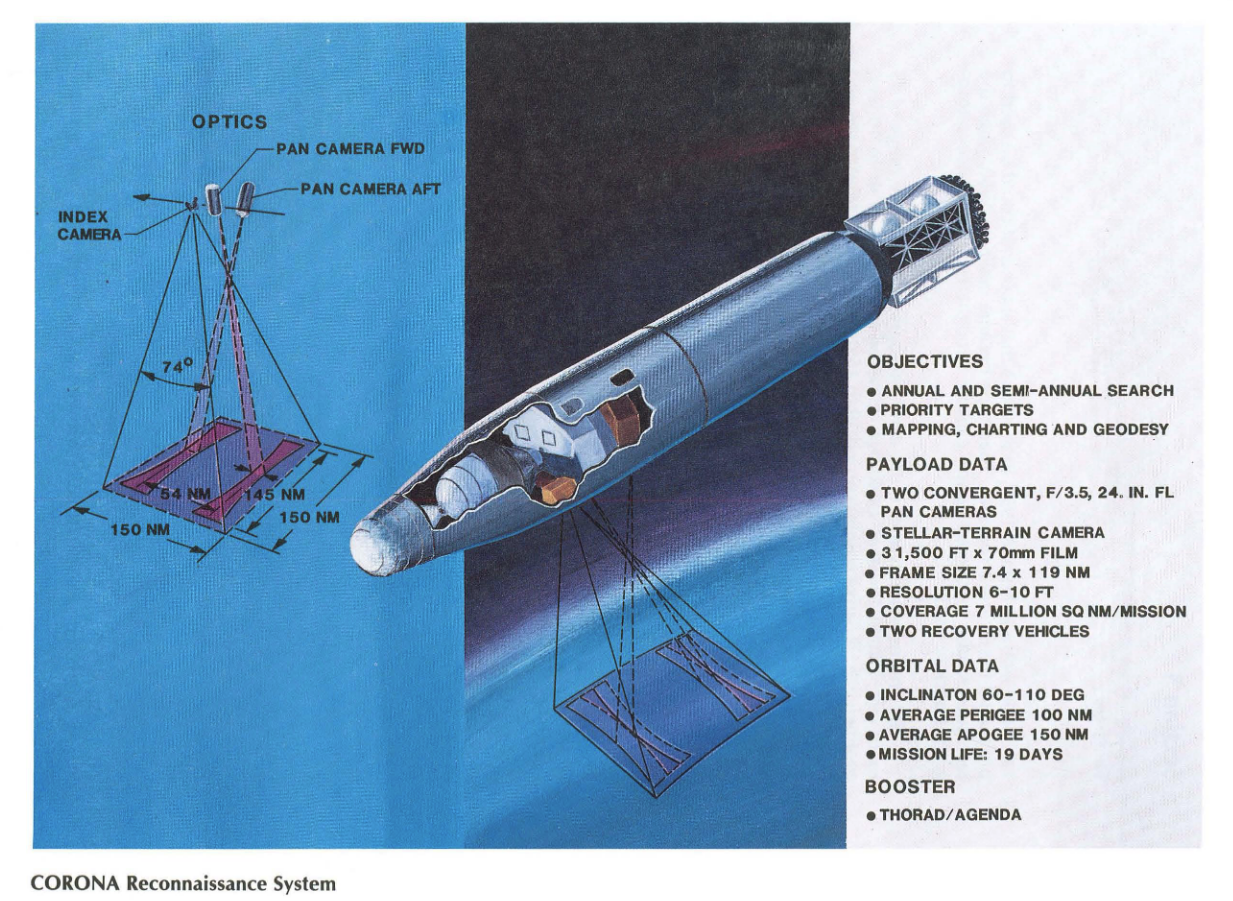
\includegraphics[totalheight=0.3\textheight]{CORONA REC .png}
\caption{CORONA Reconnaissance System's main objectives were to map, chart and survey areas of interest in enemy territories. The system is able to cover $\mathrm{2.4x10^{7}}$ km$^{2}$ per mission with a resolution of 2-3 meters \cite{CORONA}. The life of the mission is 19 days, after which the film rolled into a re-entry enclosure and jettisoned back to Earth for collection \cite{CORONA}. Photo Credits: Centre for the Study of National Reconnaissance (CSNR) and National Reconnaissance Office (NRO).
}
\end{figure}


Landsat 1 (originally named Earth Resources Technology Satellite) was launched in 1972. This was the first of many Landsat and Earth observation satellites. For the first time Landsat offered a way to observe the Earth in a repetitive and systematic way. It has contributed heavily to the understanding of Earth's environment, generated revolutionary uses of space-based data by the commercial sector and emboldened new generations of commercial and science satellites to provide high resolution spatial images of the entire Earth \cite{campbell2011introduction, Williams:2006:0099-1112:1171}.
\par
Landsat captured images in several regions of the electromagnetic spectrum, which at the time, was only available in specialised laboratories. This data popularised interests in multi-spectral analysis. Before Landsat, image analysis was performed visually by examining prints of aerial images. A second generation of instruments in the 1980s provided

\begin{figure}[H]
\centering
%\includegraphics[totalheight=0.3\textheight]{.p}
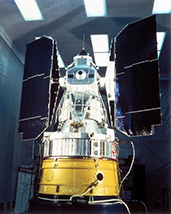
\includegraphics[totalheight=0.2\textheight]{Landsat1.jpg}
\caption{Artist's render. Landsat 1 (formerly named Earth Resources Technology Satellite ERTS-1) was launched on July 23, 1972. Photo Credits: \cite{landsat1}
}
\end{figure}


By the early $1980\mathrm{~s}$, a second generation of instruments for collecting satellite imagery provided finer spatial detail at $30-\mathrm{m}, 20-\mathrm{m}$, and $10-\mathrm{m}$ resolutions and, by the $1990 \mathrm{~s}$, imagery at meter and submeter resolutions. Finally, by the late 1990 s, development of commercial capabilities (e.g., Geoeye and IKONOS) for acquiring fine-resolution satellite imagery (initially at spatial resolutions of several meters but eventually submeter detail) opened new civil applications formerly available only through uses of aerial photography. It is important to note that such progress in the field of remote sensing advanced in tandem with advances in geographic information systems (GIS), which provided the ability to bring remotely sensed data and other geospatial data into a common analytical framework, thereby enhancing the range of products and opening new markets-mapping of urban infrastructure, supporting precision agriculture, and support of floodplain mapping, for example.


\par



To summarise, Landsat offered a way to observe the Earth in a repetitive and systematic way. It has contributed heavily to the understanding of Earth's environment, generated revolutionary uses of space-based data by the commercial sector and emboldened new generations of commercial and science satellites to provide high resolution spatial images of the entire Earth. \cite{campbell2011introduction, Williams:2006:0099-1112:1171}.

%This report will focus on cloud cover over Earth, weather forecasting and terrain identification

\subsection{EUMESAT}

Modern day remote sensing and satellite imaging goes beyond military or strategic applications. As of September 1$^{st}$ 2021, there are 4,550 known operational satellites, of which 1030 are for Earth observation \cite{Sat_Data}. Satellite imaging has a major applications in a wide range of industries from monitoring crop growth to forecasting weather. In this project, we used data from Meteosat-8 






%\subsection{Other Applications in Industry}


\subsection{Prior Work}

\subsection{Project Aims}